\chapter{Using Broadwick}

\section{Creating a New Project}\index{Creating a New Project}

Broadwick contains a set of packages that can be used as required. The framework is designed to be flexible and does not place any requirement on the user on how to use the framework. It is possible to use the classes and packages of Broadwick without using the powerful framework, creating your own main() method and taking responsibility for reading data files and configuration items though this is not the recommended way of using Broadwick.

\subsection{Using The Command Line}\index{Using The Command Line}

The Broadwick distribution contains a maven archetype for generating a skeleton project that contains all the configuration files, source code etc that is required to start a project based upon Broadwick. It uses apache maven as it’s build tool. To generate a skeleton using this archetype on the command line (assuming that the broadwick-archetype jar is in your local repository) 

\begin{sourcecode}
mvn3 archetype:generate -DarchetypeGroupId=broadwick -DarchetypeArtifactId=broadwick-archetype \
-DarchetypeVersion=1.1 -DgroupId=broadwick.proj -DartifactId=StochasticSir -Dversion=0.1 \
-Dpackage=broadwick.stochasticsir
\end{sourcecode}

The groupId (maven uses the group id to uniquely identify your project), artifactId (is the name of your generated jar file without a version), version (the version number for your generated project) and the package to which the generated source will be created can be changed by modifiying the  -DgroupId, -DartifactId, -Dversion and -Dpackage arguments above.

\subsection{Using Netbeans}\index{Using Netbeans}

It is possibly easier to create a project using Netbeans (a free IDE available form Oracle, the ‘owners’ of Java). Open the Netbeans IDE and select File->New Project and choose a Maven project and “Project from Archetype” from the list of projects (see fig{proj1}).

\begin{figure}[h]
\centering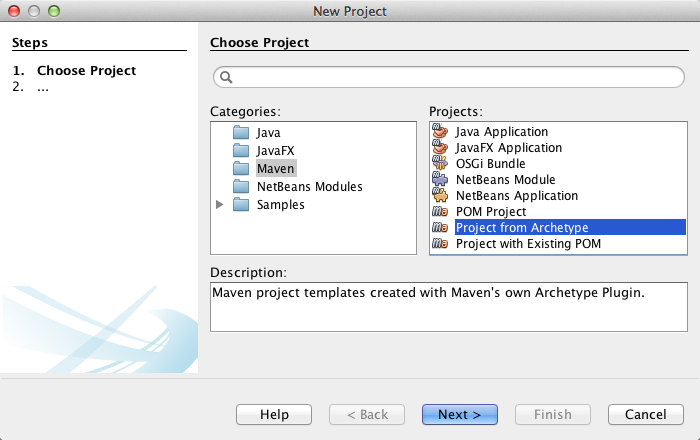
\includegraphics[width=12cm]{proj1.png}
\caption{Creating a maven based project}
\label{proj1}
\end{figure}

Click Next and choose the latest version of the broadwick-archetype from the ``Known Archetypes” (see fig \ref{proj2}). The version of the broadwick archetype corresponds to the version of Broadwick.

\begin{figure}[h!]
\centering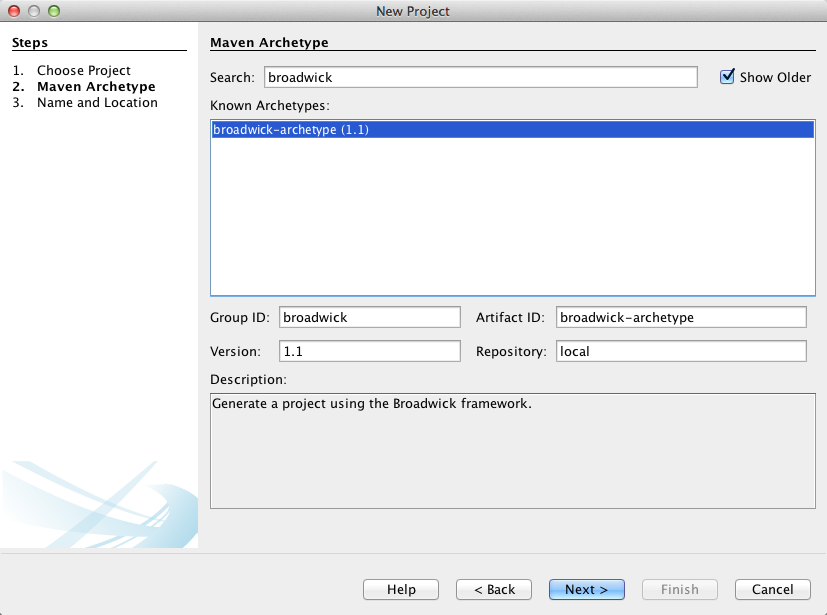
\includegraphics[width=12cm]{proj2.png}
\caption{Using the Broadwick archetype to create a skeleton project.}
\label{proj2}
\end{figure}

The projects details can be specified on the next screen (fig \ref{proj3}).

\begin{figure}[h!]
\centering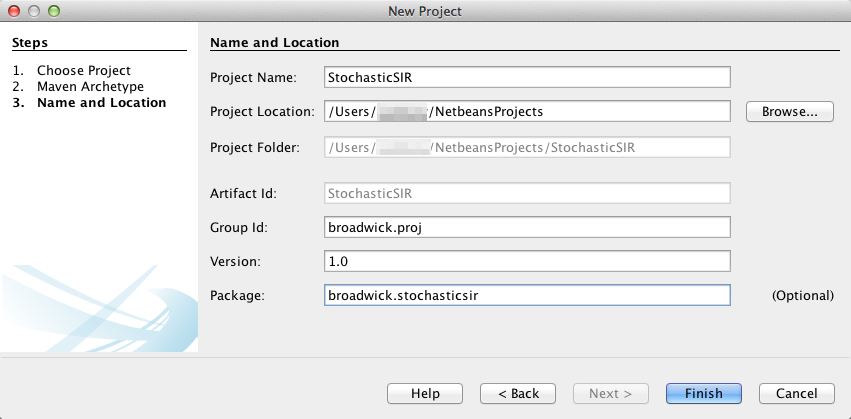
\includegraphics[width=12cm]{proj3.png}
\caption{Setting project details for a Broadwick based project.}
\label{proj3}
\end{figure}

Clicking ``Finish” will create the project (fig \ref{proj4}).

\begin{figure}[h!]
\centering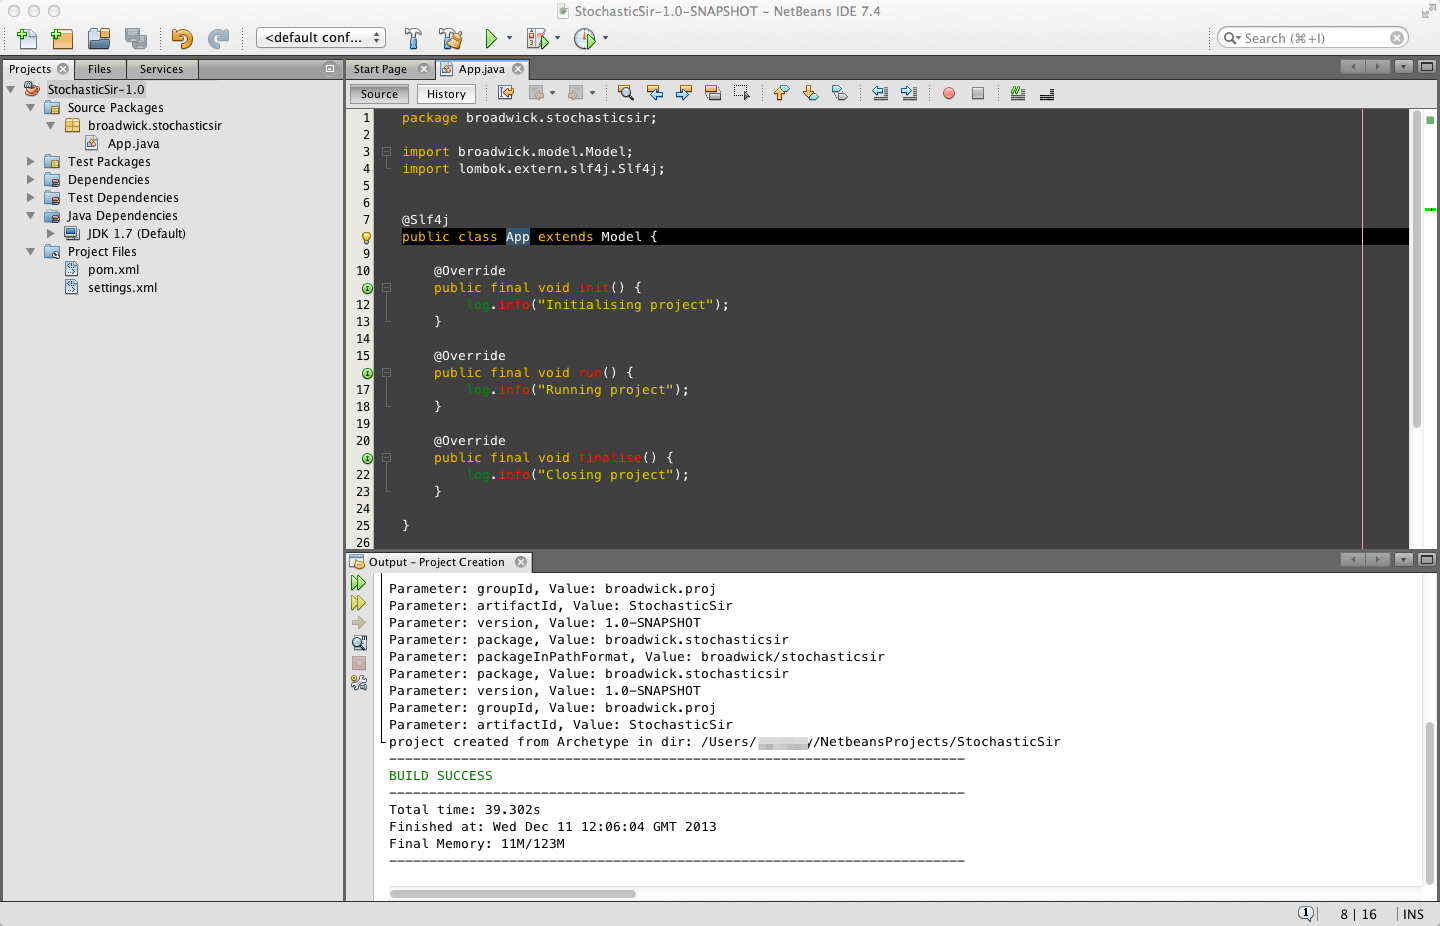
\includegraphics[width=12cm]{proj4.png}
\caption{The generated project}
\label{proj4}
\end{figure}

A number of minor changes are needed in the generated project.

Select the name of the class (``App”) and right-click and select Refactor->Rename; Change the name of the class to StochasticSIR.

In the Broadwick.sh file change the \$\{artifactId\} and \$\{version\} to the artifactId and version specified when the project was created (StochasticSIR and 1.0 respectively). This is a shell script for running your project on Unix based systems, you will need to make it executable.

In Broadwick.xml (the configuration file for the generated project) change the name of the <classname> element to reflect the package and class (broadwick.stochasticsir.StocasticSIR)

We can build the generated project by selecting Run->Build Project from the menu bar or clicking the 
\includegraphics[scale=0.22]{proj5.png} icon in the toolbar (see fig \ref{proj6} for some example output from this process). This will create a directory called target that contains, among other items, a jar file containing the compiled code and an executeable jar file ending in .one-jar.jar. The Broadwick.sh file is a shell script that will run the executable jar file on *NIX systems.

\begin{figure}[h!]
\centering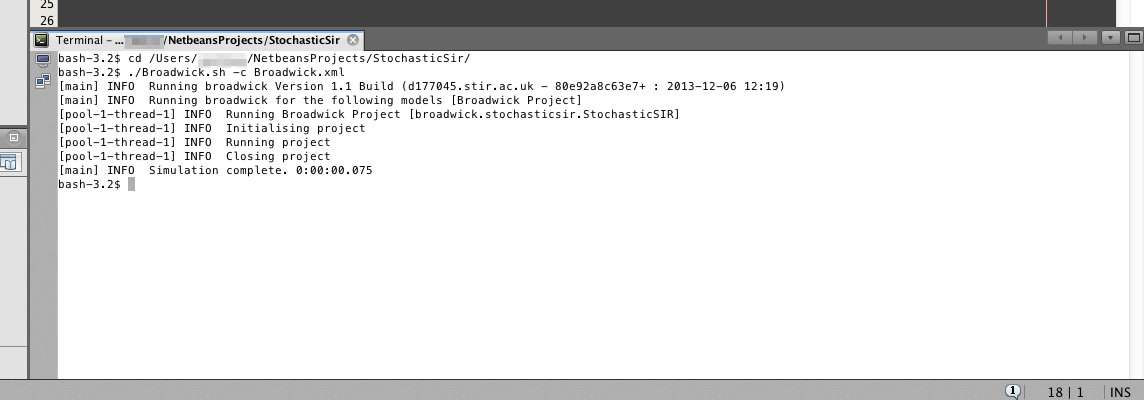
\includegraphics[width=12cm]{proj6.png}
\caption{Figure caption}
\label{proj6}
\end{figure}

When Broadwick starts it looks for all the models specified in the <model> elements in the projects configuration file. It creates objects for each <model> found using the default (empty) constructor for the class given in the <classname> element of the model (this is why no constructor is generated for the project).

For each project object created Broadwick will call the init(), run() and finalise() methods in turn. In our skeleton project we simply logged the fact that these methods were called. A simplified outline of how Broadwick initialises itself is shown in fig \ref{broadwicksummary}.

\begin{figure}[h!]
\centering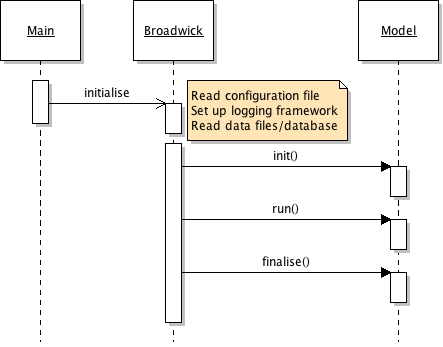
\includegraphics[width=8cm]{BroadwickSummary.png}
\caption{Schematic outline of the steps Broadwick performs on startup}
\label{broadwicksummary}
\end{figure}

A description of the configuration file is outlined in the next section.

\section{Configuration Files}\index{Configuration Files}

The configuration file MUST conform to the Broadwick.xsd specification that is supplied with the Broadwick source code. The configuration is contained within the <project> </project> tags and contains the following tags

\begin{tabulary}{1.0\textwidth}{llp{8cm}}
\toprule
<logs> & <console> & Contains <level> and <pattern> tags to define the level and structure of logging messages displayed on the console.\\
       & <files> & Contains <level> and <pattern> tags like the <console> log but also a <name> for the name of the file to contain the log messages and a boolean <overwrite> tag that lets Broadwick know if any existing file with that name should be overwritten.\\
<data> & <databases> & Contains the <name> tag to specify the location of the database.\\
       & <datafiles> & Contains the <DirectedMovementFile> <FullMovementFile> <BatchMovementFile> <PopulationFile> <LocationsFile> and <TestsFile> tags for the various file structures recognised by Broadwick. See the following tables in this section for a description of each.\\
<models> & <model> & Broadwick can run several models concurrently (though they will share the same logging and data configurations). \\
\bottomrule
\end{tabulary}

\vskip 1cm
Each model element contains the following:

\begin{tabulary}{0.3\linewidth}{l p{10cm}}
\toprule
<classname> & Exactly one classname element that is the fully qualified name of the java  class (that implements the broadwick.model.Model interface). This class MUST have a no argument constructor that Broadwick will use to create an instance through relection.\\
<priors> & The <priors> tag can contain as many elements as necessary, each prior contains an id attribute and optional <hint> and <initialVal> elements. The following priors are recognised by Broadwick\\
         & <uniformPrior> additionally contains <min> and <max> elements for uniformly distributed priors.\\
         & <gaussianprior> additionally contains <mean> and <deviation> tags for normally distributed priors.\\
         & <parameter> The parameters for the model can be encoded in this tag using the id and value attributes to name the parameters and give the parameter value. These can be accessed by the broadwick.model.Model getParameterAs[TYPE](id) method that retrieves the parameter with the given id and converts it the the required type.\\
\bottomrule
\end{tabulary}

Each datafile contains specific information on it’s layout, i.e. the columns in the file where the required data can be found. The structure of each recognised data file is outlined below.

DirectedMovementFile:

\begin{tabulary}{0.3\linewidth}{l p{9cm}}
\toprule
<name> & The name (including path from the configuration file) where the file can be found. \\
<alias> & An alias for the file. \\
<separator> & The character separating the columns in the datafile, e.g. `,' `<tab>'.\\
<idColumn> &  \\
<movementDateColumn> &  \\
<movementDirectionColumn> &  \\
<locationColumn> &  \\
<speciesColumn> &  \\
<dateFormat> &  The format the date is given in the data file, see below for details.\\
<customTags> & This optional field allows for optional information to be stored in the database. \\
\bottomrule
\end{tabulary}\\

FullMovementFile:

\begin{tabulary}{1.0\textwidth}{l p{9cm}}
\toprule
<name> & The name (including path from the configuration file) where the file can be found.\\
<alias> & An alias for the file.\\
<separator> & The character separating the columns in the datafile, e.g. `,' `<tab>'.\\
<idColumn> & \\
<departureDateColumn> & \\
<departureLocationIdColumn> & \\
<destinationDateColumn> & \\
<destinationLocationIdColumn> & \\
<marketIdColumn> & \\
<marketDateColumn> & \\
<speciesColumn> & \\
<dateFormat> & The format the date is given in the data file, see below for details.\\
<customTags> & This optional field allows for optional information to be stored in the database.\\
\bottomrule
\end{tabulary}\\

BatchMovementFile:

\begin{tabulary}{1.0\textwidth}{l p{9cm}}
\toprule
<name> & The name (including path from the configuration file) where the file can be found.\\
<alias> & An alias for the file.\\
<separator> & The character separating the columns in the datafile, e.g. `,' `<tab>'.\\
<batchSizeColumn> & \\
<departureDateColumn> & \\
<departureLocationIdColumn> & \\
<destinationDateColumn> & \\
<destinationLocationIdColumn> & \\
<marketIdColumn> & \\
<marketDateColumn> & \\
<speciesColumn> & \\
<dateFormat> & The format the date is given in the data file, see below for details.\\
<customTags> & This optional field allows for optional information to be stored in the database.\\
\bottomrule
\end{tabulary}\\

PopulationFile:

\begin{tabulary}{1.0\textwidth}{l p{9cm}}
\toprule
<name> & The name (including path from the configuration file) where the file can be found.\\
<alias> & An alias for the file.\\
<separator> & The character separating the columns in the datafile, e.g. `,' `<tab>'.\\
<lifehistory> & \\
<population> & \\
<speciesColumn> & \\
<dateFormat> & The format the date is given in the data file, see below for details.\\
<customTags> & This optional field allows for optional information to be stored in the database.\\
\bottomrule
\end{tabulary}

Lifehistory:

\begin{tabulary}{1.0\textwidth}{l p{9cm}}
\toprule
<name> & The name (including path from the configuration file) where the file can be found.\\
<alias> & An alias for the file.\\
<separator> & The character separating the columns in the datafile, e.g. `,' `<tab>'.\\
\bottomrule
\end{tabulary}

Population:

\begin{tabulary}{1.0\textwidth}{l p{9cm}}
\toprule
<name> & The name (including path from the configuration file) where the file can be found.\\
<alias> & An alias for the file.\\
<separator> & The character separating the columns in the datafile, e.g. `,' `<tab>'.\\
\bottomrule
\end{tabulary}

LocationFile:

\begin{tabulary}{1.0\textwidth}{l p{9cm}}
\toprule
<name> & The name (including path from the configuration file) where the file can be found.\\
<alias> & An alias for the file.\\
<separator> & The character separating the columns in the datafile, e.g. `,' `<tab>'.\\
<locationIdColumn> & The column in the file containing the id of the location.\\
<eastingColumn> & The column in the file containing the easting coordinate. Coordinates aren’t strictly adhered to in Broadwick so a simple y-coordinate is sufficient.\\
<northingColumn> & The column in the file containing the northing coordinate. Coordinates aren’t strictly adhered to in Broadwick so a simple x-coordinate is sufficient.\\
<dateFormat> & The format the date is given in the data file, see below for details.\\
<customTags> & This optional field allows for optional information to be stored in the database.\\
\bottomrule
\end{tabulary}

TestsFile:

\begin{tabulary}{1.0\textwidth}{l p{10cm}}
\toprule
<name> & The name (including path from the configuration file) where the file can be found.\\
<alias> & An alias for the file.\\
<separator> & The character separating the columns in the datafile, e.g. `,' `<tab>'.\\
<idColumn> & One of these is required, specifying whether the test is performed on an individual, group (e.g. herd) or location (must match the id in the Location file).\\
<groupIdColumn> & \\
<locationIdColumn> & \\
<testDateColumn> & \\
<postiveResultColumn> & \\
<negativeResultColumn> & \\
<dateFormat> & The format the date is given in the data file, see below for details.\\
<customTags> & This optional field allows for optional information to be stored in the database. \\
\bottomrule
\end{tabulary}

The date format specification follows the standard formatting for dates and times:

\begin{tabulary}{1.0\textwidth}{l p{10cm}}
\toprule
Symbol &Meaning              \\
 G     &era                  \\
 C     &century of era (>=0) \\
 Y     &year of era (>=0)    \\
 x     &year          \\
 w     &week of weekyear     \\
 e     &day of week          \\
 E     &day of week          \\
 y     &year                 \\
 D     &day of year          \\
 M     &month of year        \\
 d     &day of month         \\
 a     &halfday of day       \\
 K     &hour of halfday (0~11)      \\
 h     &clockhour of halfday (1~12) \\
 H     &hour of day (0~23)          \\
 k     &clockhour of day (1~24)     \\
 m     &minute of hour              \\
 s     &second of minute            \\
 S     &fraction of second          \\
 z     &time zone                   \\
 Z     &time zone offset/id         \\
 '     &escape for text             \\
 ''    &single quote                \\
\bottomrule
\end{tabulary}


A simplified configuration file is generated in the skeleton project. It contains configuration items for logging to console and to file for different logging levels (info, warning, error, debug, trace) and we can specify the pattern to apply to the log message.

\begin{sourcecode}
    \begin{verbatim}
<?xml version="1.0" encoding="UTF-8" standalone="yes"?>
<project>
    <logs>
        <console>
            <level>info</level>
            <pattern>[%thread] %-5level %msg %n</pattern>
        </console>
        <file>
            <name>broadwick.stochasticsir.log</name>
            <level>info</level>
            <pattern>[%thread] %-5level %msg %n</pattern>
            <overwrite>true</overwrite>
       </file>
    </logs>

    <models>
          <model id="Broadwick Project">
                 <classname>broadwick.stochsir.StochasticSIR</classname>
          </model>
    </models>
</project>
\end{verbatim}
\end{sourcecode}

Common logging patterns are:

\begin{tabulary}{1.0\textwidth}{l p{10cm}}
\toprule
\%C             & Outputs the fully-qualified class name of the caller issuing the logging request. \\
\%M  {\%method} & Outputs the method name where the logging request was issued. \\
\%L  {\%line}   & Outputs the line number from where the logging request was issued. \\
\%F  {\%file}   & Outputs the file name of the Java source file where the logging request was issued. This is not very fast and should be avoided. \\
\%d & Used to output the date of the logging event e.g. \%d{HH:mm:ss,SSS}  \\
\%m  (\%msg)    & Outputs the application-supplied message associated with the logging event. \\
\%t  (\%thread) & Outputs the name of the thread that generated the logging event. \\
\%n & Outputs the platform dependent line separator character or characters \\
\%r & Outputs the number of milliseconds elapsed since the start of the application until the creation of the logging event. \\
\%p  {\%level}  & Outputs the level of the logging event. \\
\bottomrule
\end{tabulary}


More details on logging patterns can be found at \url{http://logback.qos.ch/manual/layouts.html}.

The model section requires a <classname> giving the fully qualified class name and optional <priors> and <parameter> sections. 

\section{Extending the Model}\index{Extending the Model}

Our stochastic SIR model that we have created is a valid Broadwick model but does not perform any useful calculations. We will add some parameters to the configuration file and read (and log them) in the init() method.

Firstly, let us define beta and rho parameters for the susceptible->infectious rate and for the infectious->recovered rates respectively and parameters for the maximum time for which we will run the simulation and the name of a file in which we will save the time series data. To do this modify the configured model section by:

\begin{sourcecode}
\begin{verbatim}
<model id="Broadwick Project">
    <classname>broadwick.stochasticsir.StochasticSIR</classname>

    <parameter id="beta" value="0.2" />
    <parameter id="rho" value="0.3" />
    <parameter id="tMax" value="100" />
    <parameter id="outputFile" value="broadwick.stochasticSIR.dat" />
</model> 
\end{verbatim}
\end{sourcecode}

Now edit the init() method of the StochasticSir class as shown in fig \ref{proj7}.

\begin{figure}[h!]
\centering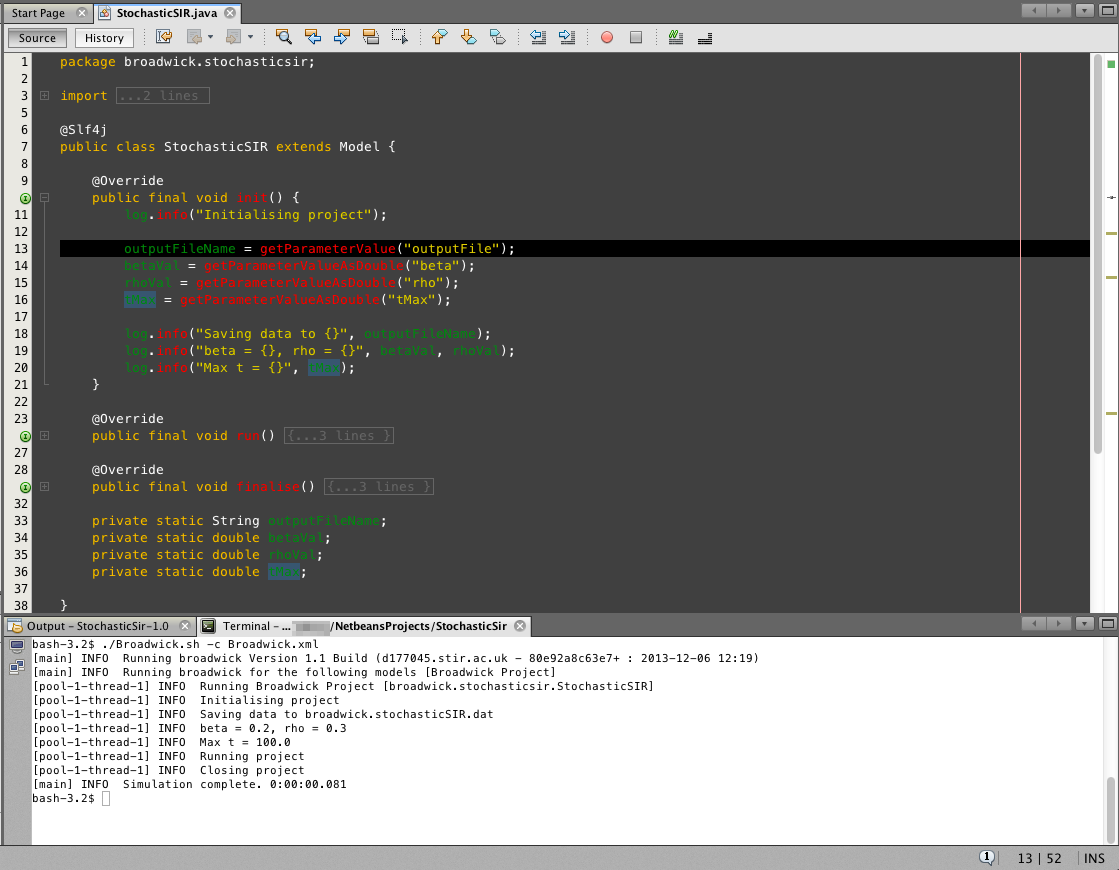
\includegraphics[width=12cm]{proj7.png}
\caption{Reading some parameters to our model}
\label{proj7}
\end{figure}

The `Model' class contains getParameterValue(String), getParameterValueAsDouble(String), getParameterValueAsInteger(String), getParameterValueAsBoolean(String) methods to extract parameters from the configuration file as strings (default), doubles, integers and booleans (if the parameter is written as ``true" or ``false").

